\subsection{UC3 - Inserimento \glossario{attività} in \glossario{EMT}}
\begin{itemize}
    \item \textbf{Identificativo}: UC3 
    \item \textbf{Nome}: Inserimento \glossario{attività} in \glossario{EMT}
    \item \textbf{Descrizione grafica}:
\end{itemize}
\begin{figure}[h]
    \centering
    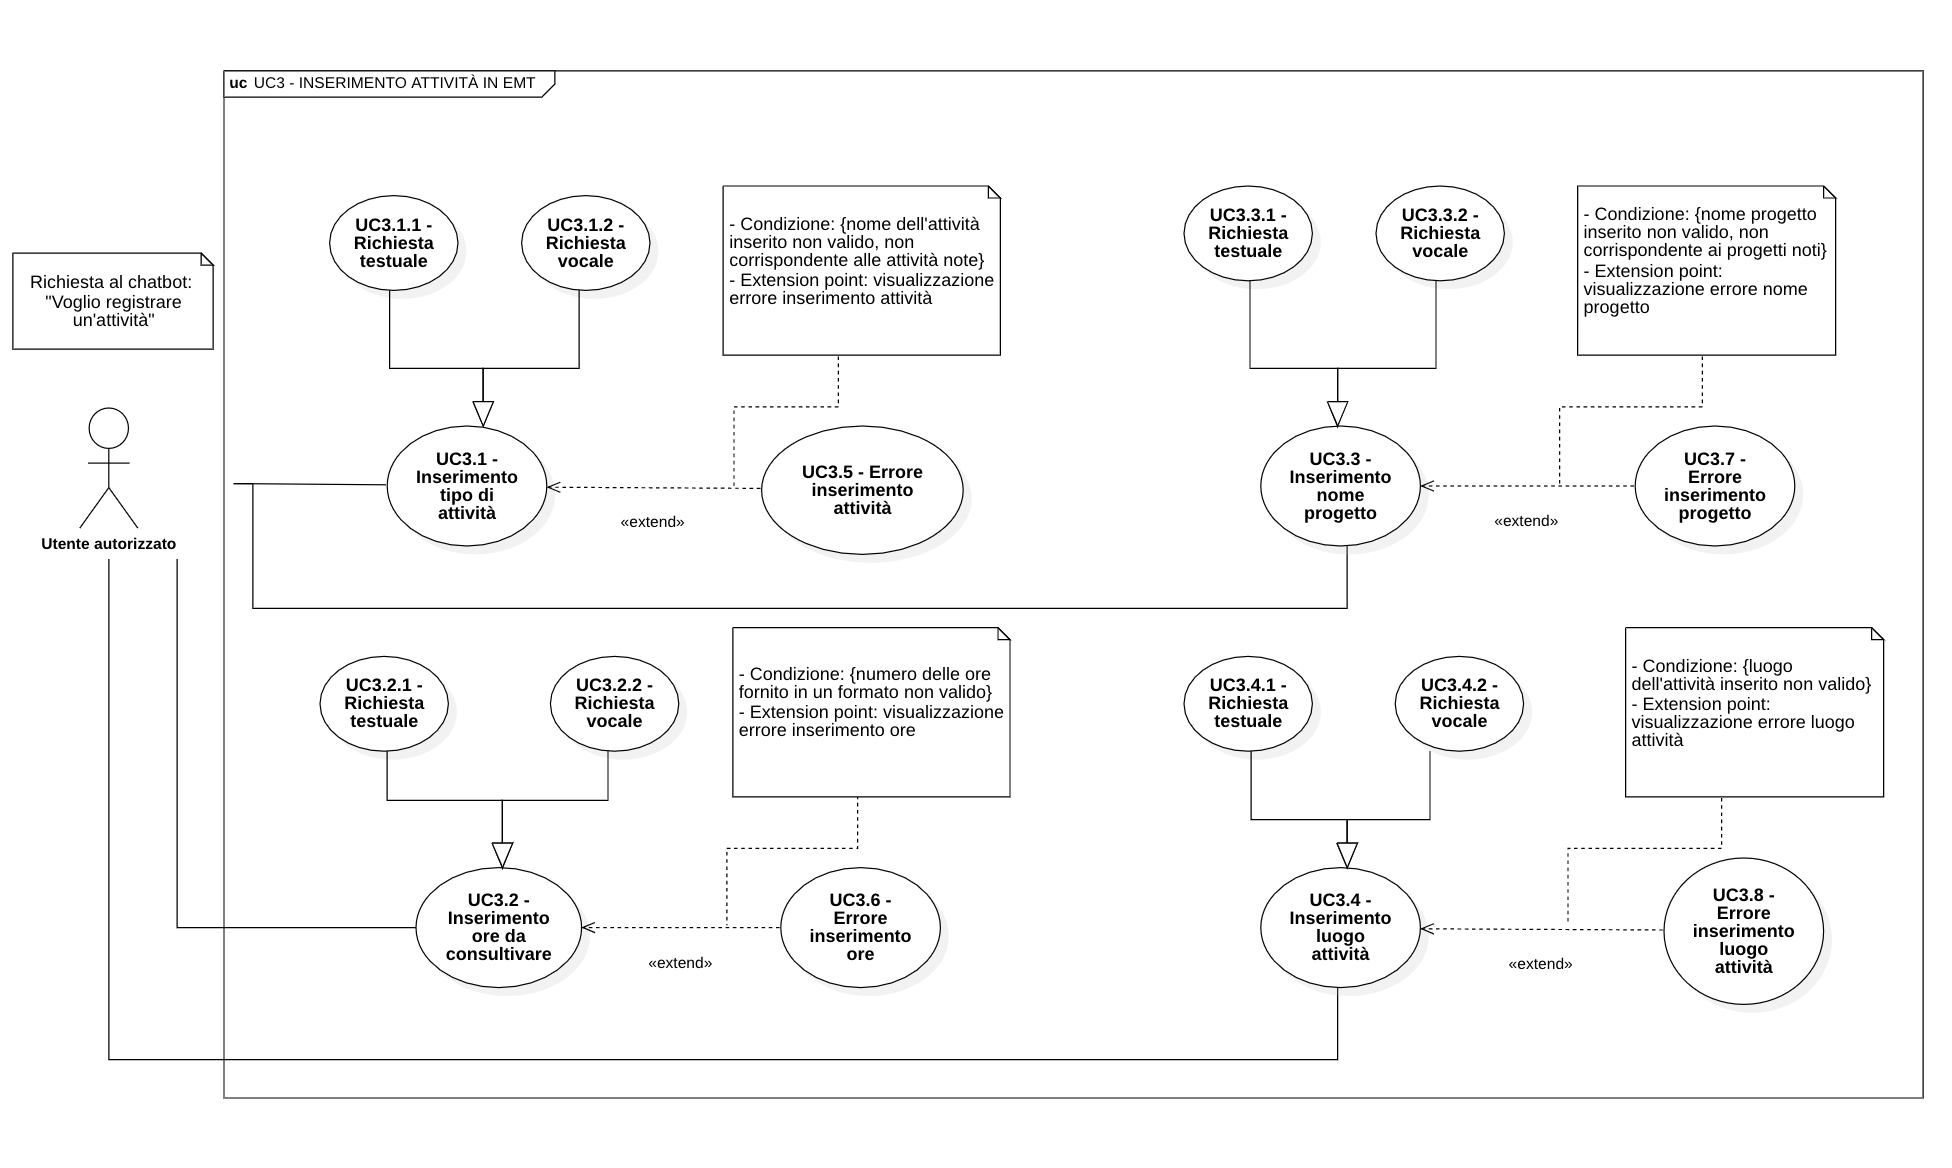
\includegraphics[scale=0.50]{images/UC3.png} 
    \caption{Descrizione grafica caso d'uso UC3}
\end{figure}

\begin{itemize}
    \item \textbf{Attori}
    \begin{itemize} 
        \item \textit{Primari}: utente autorizzato
        \item \textit{Secondari}: non presenti
    \end{itemize}
 \item \textbf{Precondizione}: l'utente si è autenticato con sucesso, si trova nella schemata in cui comunica con il chabot con l'intenzione di registrare un'attività svolta. 
 \item \textbf{Postcondizione}: l'utente è riuscito con successo ad inserire la propria attività nel sistema \glossario{EMT}.  
 \item \textbf{Scenario principale}: L'utente comunica al chatbot di voler consuntivare un'attività. Il chatbot porrà dei quesiti all'utente al fine di ottenere le seguenti informazioni: 
    \begin{itemize}
        \item L'attività che si vuole consuntivare. (UC3.1)
        \item Numero di ore che sono state necessarie per svolgere l'attività. (UC3.2)
        \item Il progetto a cui l'attività fa riferimento. (UC3.3)
        \item Il luogo dove è stata svolta l'attività. (UC3.4)
    \end{itemize}
\newpage
 Durante tale processo è possibile che si verifichino degli errori, tra cui: 
    \begin{itemize}
        \item Il chatbot segnala un errore sul progetto indicato dall'utente nel caso in cui non esista. (UC3.3)
        \item Il chatbot segnala un errore sulla sede indicata dall'utente nel caso in cui non esista. (UC3.4)
    \end{itemize}
\end{itemize}

\subsubsection{UC3.1 - Inserimento tipo di \glossario{attività}}
\begin{itemize}
    \item \textbf{Identificativo}: UC3.1 
    \item \textbf{Nome}: Inserimento tipo \glossario{attività} 
    \item \textbf{Descrizione grafica}: (approfondita in UC3)
    \item \textbf{Attori}
        \begin{itemize} 
            \item \textit{Primari}: utente autorizzato
            \item \textit{Secondari}: non presenti
        \end{itemize}
    \item \textbf{Precondizione}: l'utente ha espresso la volontà di registrare un'attività. 
    \item \textbf{Postcondizione}: l'utente ha comunicato al chatbot il tipo di attività che vuole registrare. 
    \item \textbf{Scenario principale}: L'utente comunica al chatbot il tipo di attività da consuntivare in maniera testuale (UC3.1.1) oppure vocale (UC3.1.2). L'operazione può andare a buon fine o può essere visualizzato un messaggio di errore nel caso in cui il tipo di attività non sia valido (UC3.5).
\end{itemize}

\paragraph{UC3.1.1 - Richiesta Testuale}
\begin{itemize}
   \item \textbf{Identificativo}: UC3.1.1
   \item \textbf{Nome}: Richiesta testuale
   \item \textbf{Descrizione grafica}: (approfondita in UC3)
   \item \textbf{Attori}:
   \begin{itemize} 
       \item \textit{Primari}: utente autorizzato
       \item \textit{Secondari}: non presenti
   \end{itemize}
       \item \textbf{Precondizione}: l'utente si è autenticato al sistema e ha richiesto di voler inserire un'attività nella piattaforma EMT\textsubscript{G}. 
       \item \textbf{Postcondizione}: l'utente fornisce il tipo di attività in formato testuale. 
    \item \textbf{Scenario principale}: 
       \begin{itemize}
           \item L'utente ha effettuato l'accesso al sistema 
           \item L'utente fornisce tramite input testuale il tipo di attività da  registrare
       \end{itemize}
\end{itemize}

\paragraph{UC3.1.2 - Richiesta vocale}
\begin{itemize}
   \item \textbf{Identificativo}: UC3.1.2
   \item \textbf{Nome}: Richiesta vocale
   \item \textbf{Descrizione grafica}: (approfondita in UC3)
   \item \textbf{Attori}:
   \begin{itemize} 
       \item \textit{Primari}: utente autorizzato
       \item \textit{Secondari}: non presenti
   \end{itemize}
       \item \textbf{Precondizione}: l'utente si è autenticato al sistema e ha richiesto di voler inserire un'attività nella piattaforma EMT\textsubscript{G}. 
       \item \textbf{Postcondizione}: l'utente fornisce il tipo di attività in formato vocale. 
    \item \textbf{Scenario principale}: 
       \begin{itemize}
           \item L'utente ha effettuato l'accesso al sistema 
           \item L'utente fornisce tramite input vocale il tipo di attività da  registrare
       \end{itemize}
\end{itemize}

\subsubsection{UC3.2 - Inserimento ore da consuntivare}
\begin{itemize}
    \item \textbf{Identificativo}: UC3.2 
    \item \textbf{Nome}: Inserimento ore da consuntivare  
    \item \textbf{Descrizione grafica}: (approfondita in UC3)
    \item \textbf{Attori}
        \begin{itemize} 
            \item \textit{Primari}: utente autorizzato
            \item \textit{Secondari}: non presenti
        \end{itemize}
    \item \textbf{Precondizione}: l'utente sta comunicando con il chatbot per inserire un'attività a consuntivo. 
    \item \textbf{Postcondizione}: l'utente ha comunicato le ore da consuntivare. 
    \item \textbf{Scenario principale}: all'interno dello scenario di registrazione di un'attività il chatbot chiede all'utente di inserire le ore che hanno coinvolto lo svolgimento. L'utente procede con l'inserimento dell'informazione in maniera testuale o vocale. L'operazione può andare a buon fine o può essere visualizzato un messaggio di errore nel caso in cui le ore inserite non siano valide (UC3.6).
\end{itemize}
\newpage

\paragraph{UC3.2.1 - Richiesta Testuale}
\begin{itemize}
   \item \textbf{Identificativo}: UC3.2.1
   \item \textbf{Nome}: Richiesta testuale
   \item \textbf{Descrizione grafica}: (approfondita in UC3)
   \item \textbf{Attori}:
   \begin{itemize} 
       \item \textit{Primari}: utente autorizzato
       \item \textit{Secondari}: non presenti
   \end{itemize}
       \item \textbf{Precondizione}: l'utente si è autenticato al sistema e ha richiesto di voler inserire un'attività nella piattaforma EMT\textsubscript{G}. 
       \item \textbf{Postcondizione}: l'utente fornisce il numero di ore che lo hanno coinvolto per svolgere l'attività in formato testuale. 
    \item \textbf{Scenario principale}: 
       \begin{itemize}
           \item L'utente ha effettuato l'accesso al sistema 
           \item L'utente fornisce tramite input testuale il numero di ore trascorse per svolgere l'attività
       \end{itemize}
\end{itemize}

\paragraph{UC3.2.2 - Richiesta vocale}
\begin{itemize}
   \item \textbf{Identificativo}: UC3.2.2
   \item \textbf{Nome}: Richiesta vocale
   \item \textbf{Descrizione grafica}: (approfondita in UC3)
   \item \textbf{Attori}:
   \begin{itemize} 
       \item \textit{Primari}: utente autorizzato
       \item \textit{Secondari}: non presenti
   \end{itemize}
       \item \textbf{Precondizione}: l'utente si è autenticato al sistema e ha richiesto di voler inserire un'attività nella piattaforma EMT\textsubscript{G}. 
       \item \textbf{Postcondizione}: l'utente fornisce il numero di ore che lo hanno coinvolto per svolgere l'attività in formato vocale.
    \item \textbf{Scenario principale}: 
       \begin{itemize}
           \item L'utente ha effettuato l'accesso al sistema 
           \item L'utente fornisce tramite input testuale il numero di ore trascorse per svolgere l'attività
       \end{itemize}
\end{itemize}

\subsubsection{UC3.3 - Inserimento progetto da consuntivare}
\begin{itemize}
    \item \textbf{Identificativo}: UC3.3 
    \item \textbf{Nome}: Inserimento progetto da consuntivare  
    \item \textbf{Descrizione grafica}: (approfondita in UC3)
    \item \textbf{Attori}
        \begin{itemize} 
            \item \textit{Primari}: utente autorizzato
            \item \textit{Secondari}: non presenti
        \end{itemize}
    \item \textbf{Precondizione}: l'utente sta comunicando con il chatbot per inserire un'attività a consuntivo. 
    \item \textbf{Postcondizione}: l'utente ha fornito il progetto correlato all'attività svolta al chatbot. 
    \item \textbf{Scenario principale}: l'utente tramite un messagio testuale o vocale, comunica al chatbot il nome del progetto per l'attività che sta inserendo. Tale progetto, se valido, porterà alla continuazione dell'inserimento, altrimenti il chatbot visualizzerà un messaggio di errore (UC3.7). 
\end{itemize}

\paragraph{UC3.3.1 - Richiesta Testuale}
\begin{itemize}
   \item \textbf{Identificativo}: UC3.3.1
   \item \textbf{Nome}: Richiesta testuale
   \item \textbf{Descrizione grafica}: (approfondita in UC3)
   \item \textbf{Attori}:
   \begin{itemize} 
       \item \textit{Primari}: utente autorizzato
       \item \textit{Secondari}: non presenti
   \end{itemize}
       \item \textbf{Precondizione}: l'utente si è autenticato al sistema e ha richiesto di voler inserire un'attività nella piattaforma EMT\textsubscript{G}. 
       \item \textbf{Postcondizione}: l'utente fornisce il nome del progetto sul quale ha lavorato in maniera testuale
    \item \textbf{Scenario principale}: 
       \begin{itemize}
           \item L'utente ha effettuato l'accesso al sistema 
           \item L'utente fornisce tramite input testuale il nome del progetto sul quale ha lavorato
       \end{itemize}
\end{itemize}

\paragraph{UC3.3.2 - Richiesta vocale}
\begin{itemize}
   \item \textbf{Identificativo}: UC3.3.2
   \item \textbf{Nome}: Richiesta vocale
   \item \textbf{Descrizione grafica}: (approfondita in UC3)
   \item \textbf{Attori}:
   \begin{itemize} 
       \item \textit{Primari}: utente autorizzato
       \item \textit{Secondari}: non presenti
   \end{itemize}
       \item \textbf{Precondizione}: l'utente si è autenticato al sistema e ha richiesto di voler inserire un'attività nella piattaforma EMT\textsubscript{G}. 
       \item \textbf{Postcondizione}: l'utente fornisce il nome del progetto sul quale ha lavorato in maniera vocale.
    \item \textbf{Scenario principale}: 
       \begin{itemize}
           \item L'utente ha effettuato l'accesso al sistema 
           \item L'utente fornisce tramite input vocale il nome del progetto sul quale ha lavorato
       \end{itemize}
\end{itemize}

\subsubsection{UC3.4 - Inserimento luogo \glossario{attività}}
\begin{itemize}
    \item \textbf{Identificativo}: UC3.4
    \item \textbf{Nome}: Inserimento luogo \glossario{attività}  
    \item \textbf{Descrizione grafica}: (approfondita in UC3)
    \item \textbf{Attori}
        \begin{itemize} 
            \item \textit{Primari}: utente autorizzato
            \item \textit{Secondari}: non presenti
        \end{itemize}
    \item \textbf{Precondizione}: l'utente sta comunicando con il chatbot per inserire un'attività a consuntivo. 
    \item \textbf{Postcondizione}: l'utente ha fornito al chatbot il luogo in cui ha svolto tale attività. 
    \item \textbf{Scenario principale}: l'utente tramite un messagio testuale o vocale, comunica al chatbot il luogo dove è stata svolta l'attività che sta inserendo. Tale luogo, se valido, porterà alla continuazione dell'inserimento, altrimenti il chatbot visualizzerà un messaggio di errore (UC3.8). 
\end{itemize}

\paragraph{UC3.4.1 - Richiesta Testuale}
\begin{itemize}
   \item \textbf{Identificativo}: UC3.4.1
   \item \textbf{Nome}: Richiesta testuale
   \item \textbf{Descrizione grafica}: (approfondita in UC3)
   \item \textbf{Attori}:
   \begin{itemize} 
       \item \textit{Primari}: utente autorizzato
       \item \textit{Secondari}: non presenti
   \end{itemize}
       \item \textbf{Precondizione}: l'utente si è autenticato al sistema e ha richiesto di voler inserire un'attività nella piattaforma EMT\textsubscript{G}. 
       \item \textbf{Postcondizione}: l'utente fornisce il luogo dove ha svolto l'attività in formato testuale
    \item \textbf{Scenario principale}: 
       \begin{itemize}
           \item L'utente ha effettuato l'accesso al sistema 
           \item L'utente fornisce tramite input testuale il luogo dove ha svolto l'attività
       \end{itemize}
\end{itemize}

\paragraph{UC3.4.2 - Richiesta Vocale}
\begin{itemize}
   \item \textbf{Identificativo}: UC3.4.2
   \item \textbf{Nome}: Richiesta testuale
   \item \textbf{Descrizione grafica}: (approfondita in UC3)
   \item \textbf{Attori}:
   \begin{itemize} 
       \item \textit{Primari}: utente autorizzato
       \item \textit{Secondari}: non presenti
   \end{itemize}
       \item \textbf{Precondizione}: l'utente si è autenticato al sistema e ha richiesto di voler inserire un'attività nella piattaforma EMT\textsubscript{G}. 
       \item \textbf{Postcondizione}: l'utente fornisce il luogo dove ha svolto l'attività in formato vocale.
    \item \textbf{Scenario principale}: 
       \begin{itemize}
           \item L'utente ha effettuato l'accesso al sistema 
           \item L'utente fornisce tramite input vocale il luogo dove ha svolto l'attività
       \end{itemize}
\end{itemize}

\subsubsection{UC3.5 - Errore inserimento \glossario{attività}}
\begin{itemize}
    \item \textbf{Identificativo}: UC3.5
    \item \textbf{Nome}: Errore inserimento \glossario{attività}
    \item \textbf{Descrizione grafica}: (approfondita in UC3)
    \item \textbf{Attori}
        \begin{itemize} 
            \item \textit{Primari}: utente autorizzato
            \item \textit{Secondari}: non presenti
        \end{itemize}
    \item \textbf{Precondizione}: l'utente ha fornito il nome dell'attività in un formato non valido. 
    \item \textbf{Postcondizione}: chatbot comunica all'utente la non validità dell'attività fornita.
    \item \textbf{Scenario principale}: l'utente fornisce il nome di un'attività da consuntivare che non risulta essere valido. Il chatbot notifica l'errore e chiede all'utente di riprovare l'inserimento. 
\end{itemize}

\subsubsection{UC3.6 - Errore inserimento ore}
\begin{itemize}
    \item \textbf{Identificativo}: UC3.6
    \item \textbf{Nome}: Errore inserimento ore
    \item \textbf{Descrizione grafica}: (approfondita in UC3)
    \item \textbf{Attori}
        \begin{itemize} 
            \item \textit{Primari}: utente autorizzato
            \item \textit{Secondari}: non presenti
        \end{itemize}
    \item \textbf{Precondizione}: l'utente ha fornito un numero di ore relativo all'attività in un formato non valido. 
    \item \textbf{Postcondizione}: chatbot comunica all'utente la non validità delle ore fornite.
    \item \textbf{Scenario principale}: l'utente fornisce il numero di ore di un'attività da consuntivare che non risulta essere valido. Il chatbot notifica l'errore e chiede all'utente di riprovare l'inserimento. 
\end{itemize}
\newpage

\subsubsection{UC3.7 - Errore inserimento progetto}
\begin{itemize}
    \item \textbf{Identificativo}: UC3.7
    \item \textbf{Nome}: Errore inserimento progetto
    \item \textbf{Descrizione grafica}: (approfondita in UC3)
    \item \textbf{Attori}
        \begin{itemize} 
            \item \textit{Primari}: utente autorizzato
            \item \textit{Secondari}: non presenti
        \end{itemize}
    \item \textbf{Precondizione}: l'utente ha fornito un nome di progetto relativo all'attività in un formato non valido. 
    \item \textbf{Postcondizione}: chatbot comunica all'utente la non validità del nome del progetto fornito.
    \item \textbf{Scenario principale}: l'utente fornisce il nome del progetto di un'attività da consuntivare che non risulta essere valido. Il chatbot notifica l'errore e chiede all'utente di riprovare l'inserimento. 
\end{itemize}

\subsubsection{UC3.8 - Errore inserimento luogo}
\begin{itemize}
    \item \textbf{Identificativo}: UC3.8
    \item \textbf{Nome}: Errore inserimento luogo
    \item \textbf{Descrizione grafica}: (approfondita in UC3)
    \item \textbf{Attori}
        \begin{itemize} 
            \item \textit{Primari}: utente autorizzato
            \item \textit{Secondari}: non presenti
        \end{itemize}
    \item \textbf{Precondizione}: l'utente ha fornito un luogo relativo all'attività in un formato non valido. 
    \item \textbf{Postcondizione}: chatbot comunica all'utente la non validità del luogo fornito.
    \item \textbf{Scenario principale}: l'utente fornisce il luogo dove ha svolto un'attività da consuntivare, non risultando essere valido. Il chatbot notifica l'errore e chiede all'utente di riprovare l'inserimento. 
\end{itemize}
\newpage